%% start of file `cv_german.tex', based on `template_en.tex` by Xavier Danaux (xdanaux@gmail.com).
% This work may be distributed and/or modified under the
% conditions of the LaTeX Project Public License version 1.3c,
% available at http://www.latex-project.org/lppl/.
% 
% Thomas Quaritsch <t.quaritsch@student.tugraz.at>

\documentclass[11pt,a4paper]{moderncv}

\usepackage[german]{babel}
\usepackage{moderncv-additions}

% moderncv themes
\moderncvtheme{casual}   % optional arguments are 'blue' (default), 'orange', 'red', 'green', 'grey' and 'roman' (for roman fonts, instead of sans serif fonts)
%\moderncvtheme[green]{classic}                % idem

% character encoding
\usepackage[utf8]{inputenc}                   % replace by the encoding you are using

% adjust the page margins
\usepackage[scale=0.8]{geometry}
\setlength{\hintscolumnwidth}{3cm}			  % if you want to change the width of the column with the dates
%\AtBeginDocument{\setlength{\maketitlenamewidth}{6cm}}  % only for the classic theme, if you want to change the width of your name placeholder (to leave more space for your address details

\AtBeginDocument{\recomputelengths}           % required when changes are made to page layout lengths

% personal data
\firstname{}
\familyname{}
        
%\nopagenumbers{}                             % uncomment to suppress automatic page numbering for CVs longer than one page

%----------------------------------------------------------------------------------
%            content
%----------------------------------------------------------------------------------

\begin{document}

% color redefinitions must be after \begin{document}!
%Liebherr yellow {254,180,1} black {0,0,0}
%Multivac {0, 105, 180}
%Grob {0,58,121}
\definecolor{firstnamecolor}{RGB}{0,0,0}
\definecolor{familynamecolor}{RGB}{0,0,0}
\definecolor{quotecolor}{RGB}{0, 105, 180}
\definecolor{addresscolor}{RGB}{0,0,0}
\definecolor{sectionrectanglecolor}{RGB}{0, 105, 180}
\definecolor{sectiontitlecolor}{RGB}{0, 105, 180}
\definecolor{subsectioncolor}{RGB}{0, 105, 180}
\definecolor{footersymbolcolor}{RGB}{0,0,0}

\makeatletter

%\pagestyle{empty}
%\chapter*{Bewerbungs}{unterlagen}
%
%\vspace*{50mm}
%\begin{minipage}{\textwidth}
%	\vspace*{3mm}
%	\familynamestyle{\@firstname}~~\firstnamestyle{\@familyname} 	
%	\hspace*{5mm}{{\color{firstnamecolor}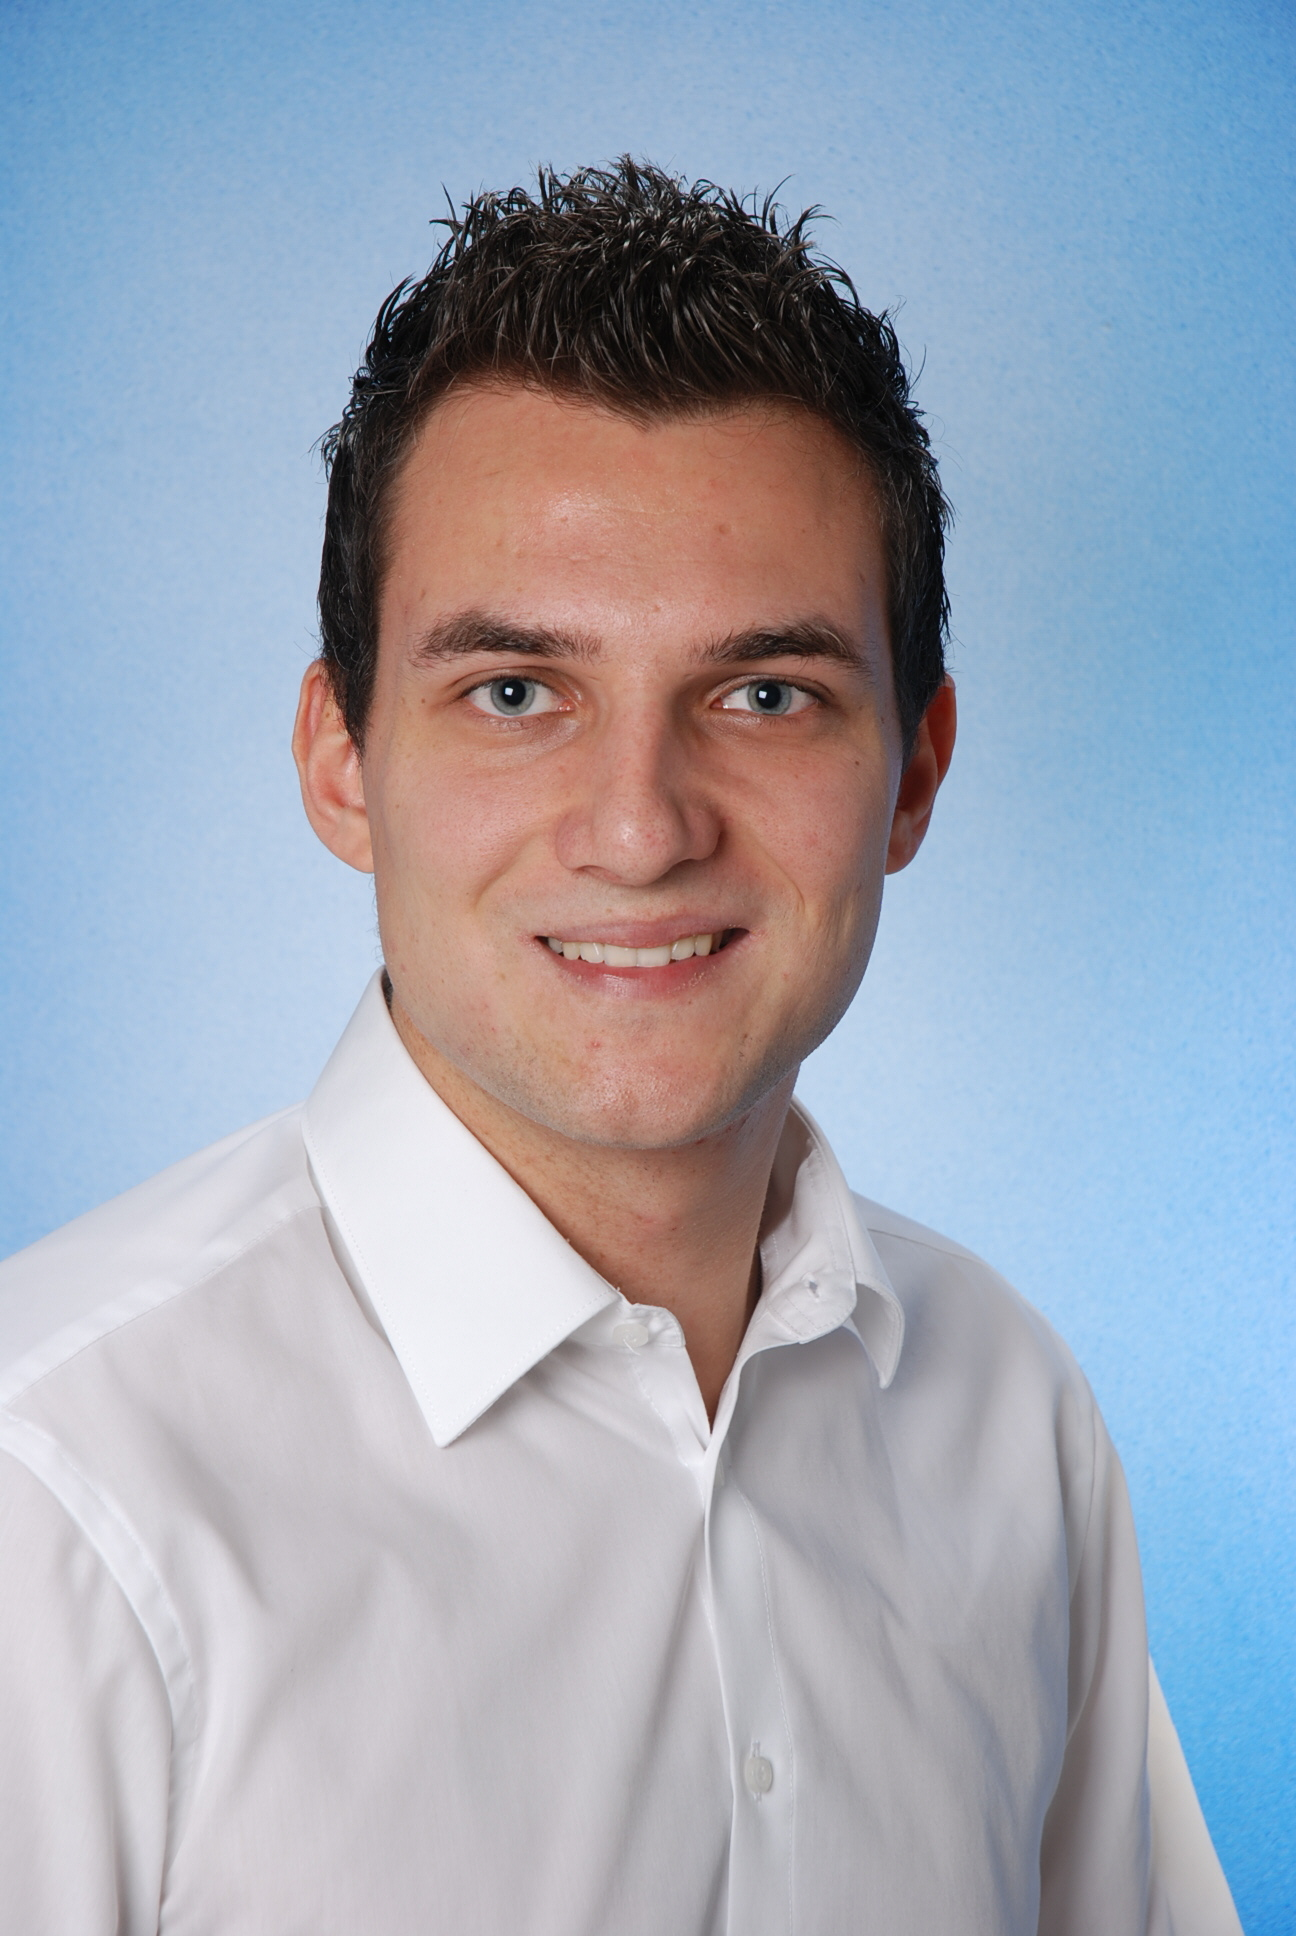
\includegraphics[width=128pt]{Anlagen/picture}}}\\[3mm]
%	\@addressstreet, \@addresscity ~~~ \mobilesymbol~\@mobile ~~~ \emailsymbol~\@email
%\end{minipage}
%\begin{minipage}{70pt}
%	
%\end{minipage}
%
%\vfill
%
%\begin{minipage}{1.0\textwidth}
%	\section{Inhalt}
%	\tableofcontents
%\end{minipage}
%
%\newpage
\pagestyle{fancy}

%\chapter{Curriculum}{~Vit\ae}
\chapter{Tätigkeitsbeschreibung}{}
%\makequote
\\
Meine aktuelle Tätigkeit als Softwareentwickler bei der Liebherr Verzahntechnik GmbH.\\
Beschäftigungsdauer: 06/2018 bis heute (nicht gekündigtes Arbeitsverhältnis)\\

\section{Projektleitung für das Produkt  Depalettieren} 
%%%%%%%%%%%%%%%%%%%%%%%%%%%%%%%%%%%%%%%%%%%%%%%%%%%%%%%%%%%%%%%%%%%%
Ziel des Entwicklungsprojektes für das Produkt Depalettieren war es, ein standardisiertes Vision-System zur Erkennung von Bauteilen bei klassischen Depalettier-Anwendungen zu ermitteln. Hierfür arbeitete ich mich zunächst in die Thematik ein und ermittelte die Anforderungen an das Produkt zusammen mit Vertrieb und Produktmanagement. Anschließend entwickelte ich technische Lösungsvorschläge, welche abteilungsübergreifend mit der Geschäftsführung abgestimmt wurden. Die beschlossenen Lösungsansätze wurden dann von mir mittels eigens erstellten Testszenarien geprüft und die dazu nötigen Systemkomponenten ermittelt. Nach dem Reporting der gesamten Projektparameter und des finalen Systems an die Geschäftsleitung wurde das Projekt erfolgreich und innerhalb des vorgegebenen Budgets 2021 abgeschlossen. Bis heute betreue ich aktiv Kundenprojekte und -tests, welche dieses Produkt betreffen.

\section{Softwareentwicklung LHRobotics.Vision} 
%%%%%%%%%%%%%%%%%%%%%%%%%%%%%%%%%%%%%%%%%%%%%%%%%%%%%%%%%%%%%%%%%%%%
LHRobotics.Vision ist eine Software zur Ermittlung der Lage von chaotisch angeordneten Bauteilen auf Basis von 3D-Sensordaten. Die C++ basierte Software wurde initial vom Fraunhofer Institut IPA entwickelt und von der Liebherr Verzahntechnik GmbH für Kundenprojekte eingesetzt, bis sich Liebherr dazu entschloss selbst in die Entwicklung einzusteigen. Ziel der Übernahme war es, die Software industrietauglich zu machen und diese auch als Standalone-Version zu vermarkten. Meine Aufgabe war es zunächst den Übergabeprozess der Software von Fraunhofer zu Liebherr zu koordinieren und mich mit Hilfe des Fraunhofer Instituts in den Quellcode einzuarbeiten. Anschließend ermittelte ich im Entwicklungsteam die ersten Anforderungen zur Verbesserung der Software und setzte diese erfolgreich um. Bis heute konnten wir eine erhebliche Verbesserung der Software in Punkten wie Bedienbarkeit, Stabilität und Performance erzielen, was uns interne und externe Anwender bestätigen. Bis heute arbeiten wir an weiteren Verbesserungen und neuen Features für die Software. Neben den Entwicklungstätigkeiten übernehme ich auch die technische Durchführung von Kundenprojekten und Machbarkeitsanalysen. Somit bin ich gleichzeitig als Anwender der Software aktiv und erkenne dadurch potentielle Verbesserungsmöglichkeiten selbst.

\section{Vermarktung LHRobotics Vision} 
%%%%%%%%%%%%%%%%%%%%%%%%%%%%%%%%%%%%%%%%%%%%%%%%%%%%%%%%%%%%%%%%%%%%
LHRobotics.Vision wurde zunächst nur für die Umsetzung schlüsselfertiger Automationsanlagen für Endkunden genutzt. In Zukunft soll die Software auch direkt an Endkunden angeboten werden, damit diese die Software selbstständig in ihre eigenen Automantionsanlagen integrieren können. Ziel des Vermarktungs-Projektes ist es ein Konzept zu entwickeln, um die Software als Standalone verkaufsfähig zu machen. Auch hierbei nehme ich eine leitende Rolle ein, koordiniere die Anforderungen von Produktmanagement und Vertrieb, erstelle Schulungs- und Dokumentationskonzepte und ermittle noch fehlende Verkaufs-Features wie beispielsweise den Lizenzschutz, welche ich dann selber implementiere. Das Projekt ist aktuell noch im Gange.

\newpage

\section{Projektleitung Forschungsprojekt Sim4Dexterity} 
%%%%%%%%%%%%%%%%%%%%%%%%%%%%%%%%%%%%%%%%%%%%%%%%%%%%%%%%%%%%%%%%%%%%
Die Liebherr Verzahntechnik ist einer der Projektpartner bei dem vom BMBF geförderten Forschungsprojekt Sim4Dexterity. Ziel dieses Projektes ist die Erzeugung synthetischer Daten für die Robotermanipulation mit hochwertigen, interaktiven und validierbaren Simulationswerkzeugen. Hierbei bin ich für die Projektleitung seitens Liebherr verantwortlich. Als Projektleiter bin ich zunächst der zentrale Ansprechpartner für interne und externe Nachfragen übernehme die bürokratische Verantwortung bei der Erstellung von Anträgen, offiziellen Dokumenten und auch deren Inhalten, wie geplanten Budgets und Zeitaufwendungen. Zusätzlich bin ich ebenfalls als durchführender Mitarbeiter bei den Entwicklungsarbeiten aktiv, wie beispielsweise der Erstellung von Simulationsmodellen und deren Programmierung innerhalb der verwendeten Simulationsumgebung. Zwischenergebnisse reporte ich in festgelegten Abständen der internen Geschäftsführung und dem externen Projektträger.
\end{document}

% end of file `cv_german.tex'